\documentclass[12pt]{article}
\usepackage[utf8]{inputenc}
\usepackage{geometry}
\usepackage{graphicx}
\usepackage{parskip}
\usepackage{amsmath}
\usepackage{hyperref}
\usepackage{titlesec}
\usepackage{float}

\geometry{a4paper, margin=1in}

\title{\bf About My Home Town: Project Plan \\ \large CSC478: Software Engineering Capstone}
\author{Audrey Yates, William Morgan, Steven Hogue \\ Group 11}
\date{\today}

\begin{document}

\maketitle

\tableofcontents

\newpage

\section{Scope Statement}\label{sec:scope}

\subsection{Overview}

Our website will be viewable at \href{https://www.aboutmyhometown.com}{https://www.aboutmyhometown.com}.

We will construct a cross-platform web application that allows users to check on a variety of data points for their locale. This data may include, but is not limited to, gas prices, current and forecast weather, restaurant/food prices, public facilities, local businesses, and possibly crime information. The goal is to compile as much data from public or low-cost API's into a single interface, adding statistical analysis, and overlaying it into a mapping application (such as Google Maps). As a long-term goal we would like to interpret and nd news articles relating to an area of interest, and pin the location in which they took place on the map.

\subsection{Platform}

This interface will be available through any modern, commonly used web browser. As the application is a web application, an internet connection and a modern browser is all that is required. The goal is to allow it to look good and work on a wide range of OS's and devices.

\subsection{Infrastructure}

The tech stack for this project will include Angular for front end development, a GitHub repository for project storage and CI/CD, online JIRA (team.atlassian.com) for ticket tracking, with the primary infrastructure being hosted in AWS.

\textbf{Project Management:}

\begin{itemize}
    \item \textbf{GitHub:} Project CI/CD pipelines and code versioning
    \item \textbf{Jira:} Team, work, and project tracking
\end{itemize}


\textbf{Tech stack:}
\begin{itemize}
    \item \textbf{Angular:}  Front-end and interface development
    \item \textbf{Bootstrap:} Easy-to-use and cross platform formatting engine
    \item \textbf{AWS:} Hosting and server resources
          \begin{itemize}
              \item{\bf S3}: Static website host
              \item{\bf Lambda}: Server-side processing, done primarily in Python
              \item{\bf Database}: MySQL and DynamoDB, for handling long-term storage of users and fast-changing API data respectively
              \item{\bf API Gateway}: Handle traffic and routing management
              \item{\bf Certificate Manager}: Ensure up-to-date SSL certificate
              \item{\bf Route 53}: DNS server
              \item{\bf CloudFront}: High speed performant content delivery network (CDN)
              \item{\bf CloudFormation}: Used to configure the cloud resources from managed templates
          \end{itemize}
\end{itemize}

\subsection{Integrations}

Our plan will need to integrate with a number of other web services, including lots of data gathering APIs. Other APIs will include a map API such as OpenStreetMap or Google Maps, pending available functionality.
User registration and login will be required, with each user specifying their location (see Timeline). Parts of the authentication will be stored both in browser local storage and the database.

\subsection{Programming Languages}

This project will use TypeScript (Angular), HTML, and CSS for the frontend user interface, with Python being used in Lambda functions as the server-side processor. It will also include SQL for database management, and AWS specific CloudFormation templates for infrastructure management.

\subsection{Timeline}

The initial focus will be on the Springfield area until the product is refined. Once that is satisfactory, if time permits, we would like to expand the scope to include other areas in Illinois or further. The goal is to make the site work dynamically based on the user's location, though that could end up being too complicated as available data reaches its limits.

\section{Organization Chart}

\textbf{Frontend Design:} Audrey Yates \\
Design the user interface, including the layout, color scheme, and overall look of the application.

\textbf{API Integrations:} Bill Morgan \\
Integrate the various APIs that will be used to gather data for the application.

\textbf{Architecture:} Steven Hogue \\
Implement the overall architecture of the application, including the database, user authentication, and CI/CD.

\section{Gantt Chart}

\begin{figure}[H]
    \centering
    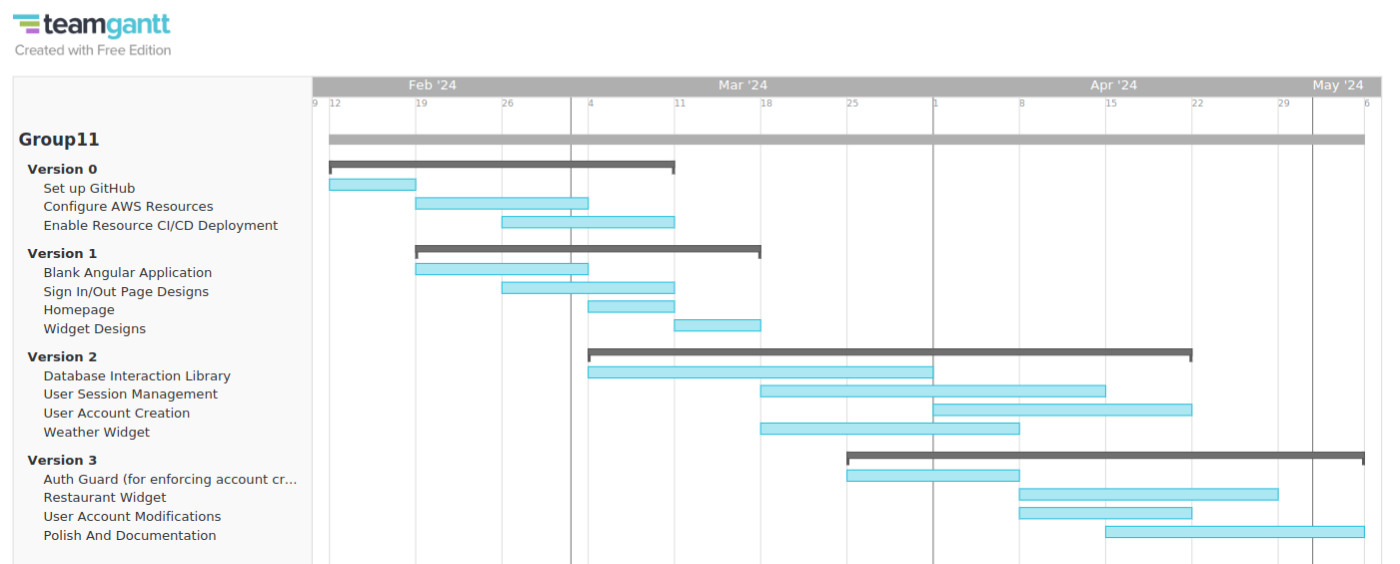
\includegraphics[width=\textwidth]{images/gantt_chart.png}
    \caption{Gantt Chart}
\end{figure}

\section{Tools and Standards}

\subsection{Development}
\subsubsection{Tools}

\begin{itemize}
    \item \textbf{NodeJS:} 20.0.0+
          \begin{itemize}
              \item The core for building the application
          \end{itemize}
    \item \textbf{Angular:} 14.3.0+
          \begin{itemize}
              \item The architecture that the application will be built on
          \end{itemize}
    \item \textbf{Python:} 3.11.0+
          \begin{itemize}
              \item Needed for some of the Lambda functionionality
          \end{itemize}
    \item \textbf{Docker:} 26.1.0+
          \begin{itemize}
              \item Needed in order to run the application locally, primarily for use with the AWS SAM CLI in deploying local copies of the Lambda functions
          \end{itemize}
    \item \textbf{AWS SAM CLI:} 1.113.0+
          \begin{itemize}
              \item Prefered command line utility for all deployments to AWS, and local testing of Lambda functions
          \end{itemize}
\end{itemize}

\subsubsection{Applications}

\begin{itemize}
    \item \textbf{VS Code}
          \begin{itemize}
              \item The code editor and IDE of choice for our team
          \end{itemize}
    \item \textbf{Google Chrome or Mozilla Firefox}
          \begin{itemize}
              \item These are the browsers that the application will be tested on by default
          \end{itemize}
\end{itemize}

\subsection{Standards}
\begin{itemize}
    \item \textbf{Python PEP 8 Style Guide}
    \item \textbf{Agile Development}
\end{itemize}

\section{Configuration Management}

\subsection{GitHub}
The project will be stored in a GitHub organization, with the main branch being the primary branch for the project. All changes will be made in feature branches, and merged into the master branch via pull requests. The project will be built and deployed via GitHub Actions.

For release management, the project will use GitHub releases to track the progress of the project, and to mark major milestones. This will be done simultaneously using tags and releases.

\textbf{GitHub Organization:} \href{https://github.com/AboutMyHT}{https://github.com/AboutMyHT}

\textbf{Angular Application Repository:} \href{https://github.com/AboutMyHT/angular-app}{https://github.com/AboutMyHT/angular-app}

\textbf{AWS Resources Repository:} \href{https://github.com/AboutMyHT/aws-resources}{https://github.com/AboutMyHT/aws-resources}

\end{document}
